\xsection{myblue}{Research question}

\begin{frame}
  \frametitle{$g_{HZZ}$ - What can be gained?}
  Extracted from Higgsstrahlung events at a $\sqrt{s}=250$~\GeV.
  \begin{columns}[c,onlytextwidth]
  \begin{column}{0.60\textwidth}
  \begin{itemize}
    \item $Z \rightarrow \mu^+ \mu^-, Z \rightarrow e^+ e^-$:
          Golden channels.

          Recoil mass method, already {\color{llblue}
            \href{https://arxiv.org/abs/1604.07524}{studied elsewhere.}}
    \item $Z \rightarrow \tau^+ \tau^-$:
        Tagging on the $\tau$ is complicated.
        \begin{itemize}
          \item Large $\tau$ decay opening angle (low $E_\tau$).
          \item Divers environment from the Higgs decay.
        \end{itemize}
    \item $Z \rightarrow \nu\bar{\nu}$:
      \begin{itemize}
        \item[--] Significant WW-fusion contribution in $\nu\bar{\nu}H$.
        \item[--] Cannot tag event on $\nu$.
        \item[+]  Only Higgs boson (and beam overlay)

            present in event.
        \item[+]  $6\times$ higher cross section.
      \end{itemize}
  \end{itemize}
  \end{column}
  \begin{column}{0.40\textwidth}
    \resizebox{\textwidth}{!}{
      % Define styles for the different kind of edges in a Feynman diagram
\tikzset{
    vector/.style={decorate, draw=black,
    decoration={snake, segment length=4mm, amplitude=1mm}},
    fermion/.style={draw=black, postaction={decorate},
        decoration={markings,mark=at position .55 with {\arrow[draw=black]{>}}}},
    fermionbar/.style={draw=black, postaction={decorate},
        decoration={markings,mark=at position .55 with {\arrow[draw=black]{<}}}},
    gluon/.style={decorate, draw=black,
        decoration={coil,amplitude=4pt, segment length=5pt}},
    higgs/.style={dashed,draw},
    photon/.style={decorate, decoration={snake}, draw=black},
    electron/.style={draw=black, postaction={decorate},
        decoration={markings,mark=at position .55 with {\arrow[draw=black]{>}}}},
    positron/.style={draw=black, postaction={decorate},
        decoration={markings,mark=at position .55 with {\arrow[draw=black]{<}}}}
}


\begin{tikzpicture}[line width=1.5pt, scale=1]
    \node (i1 e+) at (-140:2) {};
    \node (v4 ISR) at (-140:1.5) {};
    \begin{scope}[shift={(v4 ISR)}]
        \node (f4 gamma) at (10:1.5) {};
    \end{scope}
    \node (i2 e-) at (140:2) {};

    \node (v1 eeZ) at (0,0) {};
    \node (v2 ZZH) at (0:2) {};
    \begin{scope}[shift={(v2 ZZH)}]
        \node (v3 Zll) at (-40:1.5) {};
        \node (f1 H) at (40:1.6) {};
    \end{scope}
    \begin{scope}[shift={(v3 Zll)}]
        \node (f3 l-) at (-60:2) {};
        \node (f2 l+) at (-20:2) {};
        \node (v5 FSR) at (-20:0.5) {};
    \end{scope}
    \begin{scope}[shift={(v5 FSR)}]
        \node (f5 gamma) at (0:1.5) {};
    \end{scope}
    \begin{scope}[shift={(f3 l-)}]
        \node (f6 nu tau) at (-10:1.5) {};
        \node (f7 W) at (10:1.5) {};
    \end{scope}

    
    \draw[fermionbar] (i1 e+)--(v1 eeZ.center);
        \node at (i1 e+) {$e^+$};
    \draw[fermion] (i2 e-)--(v1 eeZ.center);
        \node at (i2 e-) {$e^-$};

    \draw[vector] (v1 eeZ.center)--(v2 ZZH.center);
        \node at ($ 0.5*(v1 eeZ) + 0.5*(v2 ZZH)  + (0,0.3) $) {$Z$};
    \draw[vector] (v2 ZZH.center)--(v3 Zll.center);
        \node at ($ 0.5*(v2 ZZH) + 0.5*(v3 Zll)  + (0.2,0.2) $) {$Z$}; % = midpoint of propagator + fine tuning	
    \draw[higgs] (v2 ZZH.center)--(f1 H);
        \node at (f1 H) {$H$};	

    \draw[vector] (v4 ISR.center)--(f4 gamma);
    \node at (f4 gamma) {$\gamma$};

    \draw[fermion] (v3 Zll.center)--(f3 l-);
    \draw[fermionbar] (v3 Zll.center)--(f2 l+);

    \node at (f3 l-) {$f$};
    \node at (f2 l+) {$\bar{f}$};    
    
\end{tikzpicture}
    }
  \end{column}
  \end{columns}
  \end{frame}


\begin{frame}
  \frametitle{\texorpdfstring{{$\nu\bar{\nu}H$}}{vvH}}
  \begin{columns}[c,onlytextwidth]
  \begin{column}{0.55\textwidth}
  \begin{itemize}
    \item $\sigma_{\nu\bar{\nu}H}$ with contributions from both Higgsstrahlung
        and WW-fusion.
    \item Their relative size varies with the beam polarisation.
    \item Similar distributions for $\sqrt{s}=250~\GeV$.
    \item Idea: Extract the combined cross section

        ($\rightarrow$ production mode agnostic selection).
    \item WIP: Determine the benefit of this observable for $G_{HZZ}, G_{HWW}$
        from a global fit, including the correlations with e.g.
        $\sigma_{\tn{WW-fusion} \rightarrow \nu\bar{\nu} b\bar{b}}$

        (using {\color{llblue}\href{https://arxiv.org/abs/1706.02174}{SFitter}}).
  \end{itemize}
  \end{column}
  \begin{column}{0.45\textwidth}
  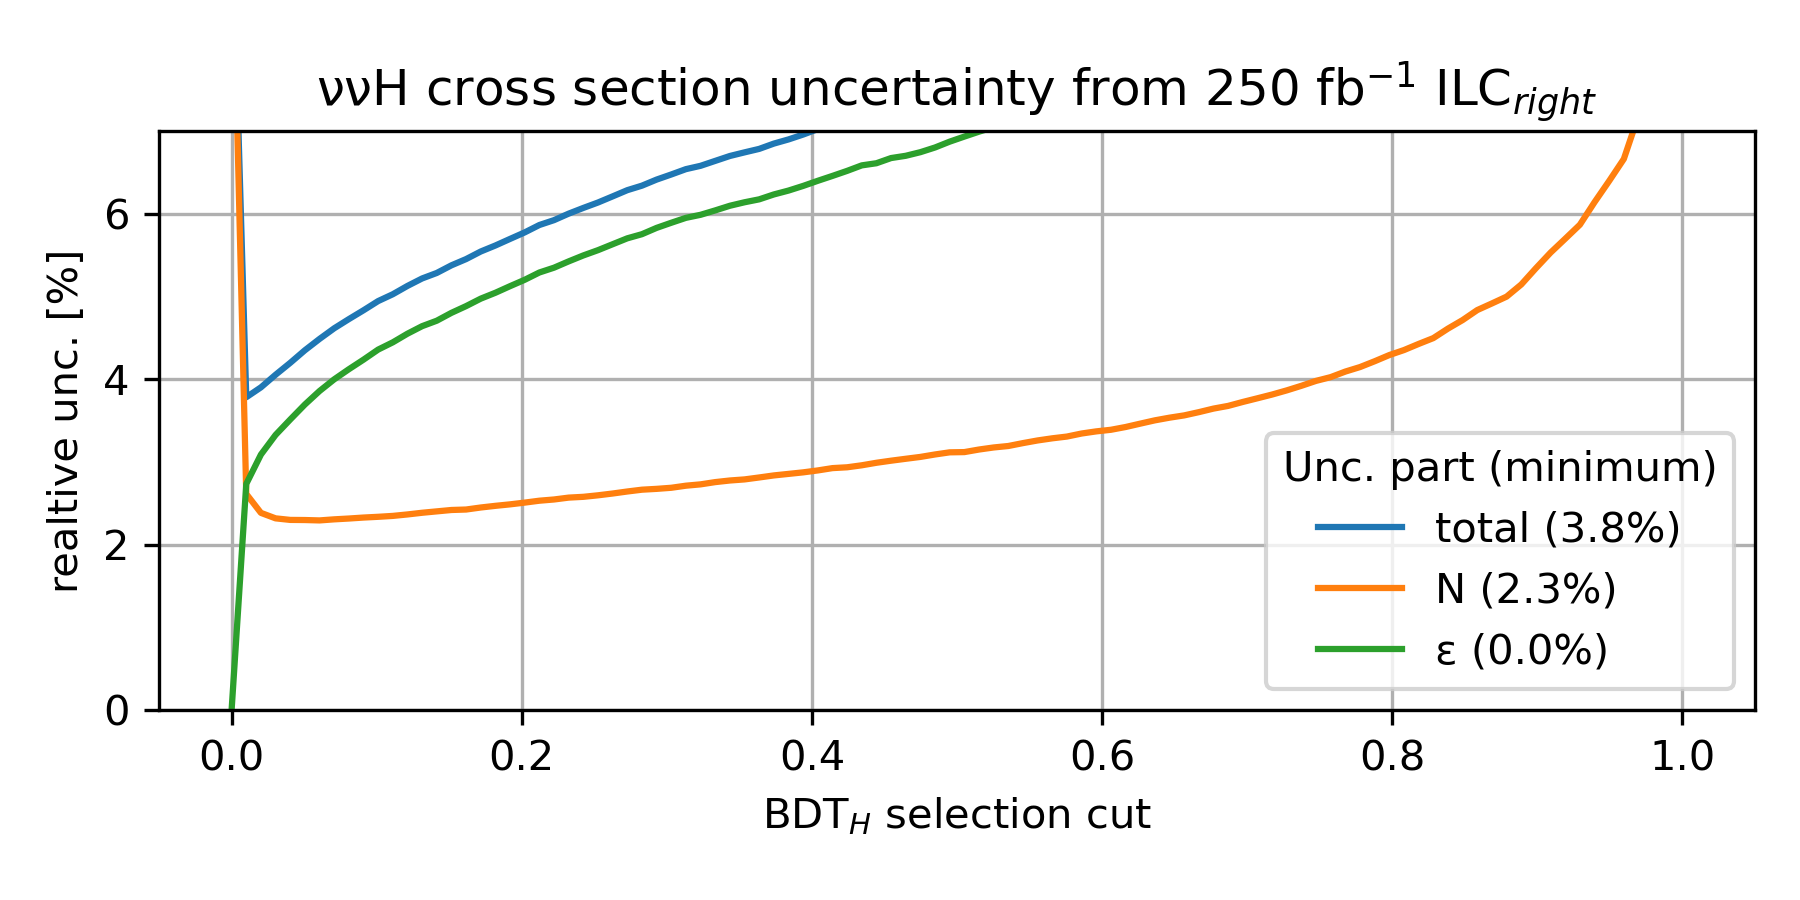
\includegraphics[height=0.5\textheight, width=0.8\textwidth, keepaspectratio]
      {ext_nnH_cs_uncertainty}
  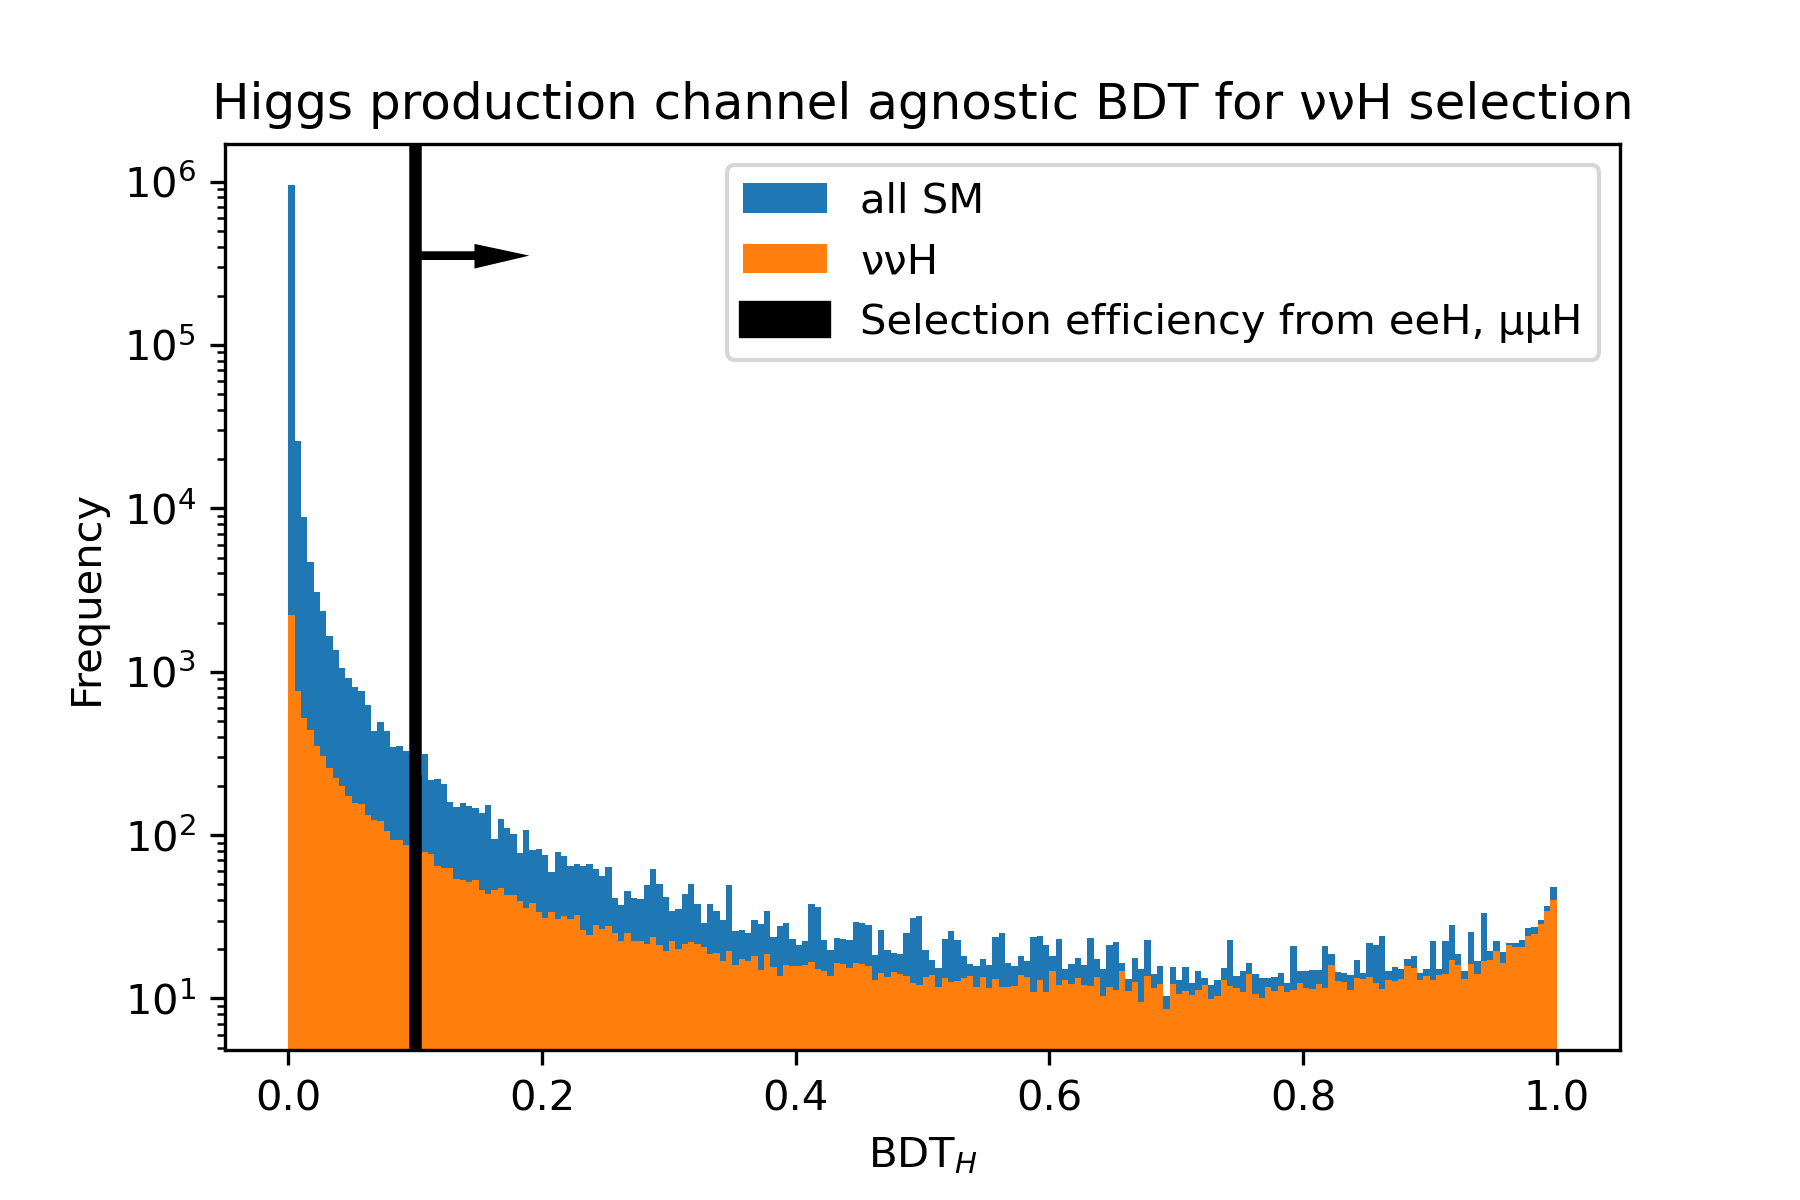
\includegraphics[height=0.7\textheight, width=\textwidth, keepaspectratio]
      {ext_nnH_BDT_production_agnostic}
  \end{column}
  \end{columns}
  \end{frame}